\section{Changes to architecture to allow vector operations.}

To perform the vector operations in a single clock cycle extra ALUs had to be added. These ALUs were placed in parallel with the original and each output into its own accumulator. Originally it had been intended that the accumulators would each output onto one 16n wide bus where n was the number of ALUs present in the system. This design ran into issues however due to the physical limitations of the memory units on the FPGA. These ram blocks could only support 32 bits being written and read per clock cycle. This limited the CPU to either two ALUs or multiple clock cycles per vector operation to access the memory. Both of these options would have resulted in a significant reduction to the maximum speed up obtainable by the CPU over the original design and so another solution was looked for.

This solution came in the form of using dedicated ram for each ALU. This lack of shared ram however introduced a new problem, there was no longer any way for the ALUs to read what was written to the others memory. This problem was solved via the modification of the load store instructions. Initially these instructions used an 8 bit operand to address the I/O to send and receive from. This was broken up into one 4 bit address operand and one 4 bit memory operand. For the load operation if the operand was one of the memory addresses the value of the addressed data memory would be loaded into the accumulator of all the ALUs through the use of a new data select register. If a store instruction was used then the output of the addressed ALUs accumulator register would be stored to its memory. This effectively allowed for data to be moved between the data memories. A block diagram of the modification to the modifications to the data path mentioned can be seen in Figure~\ref{new_path}

\begin{figure*}[ht]
	\begin{center}
		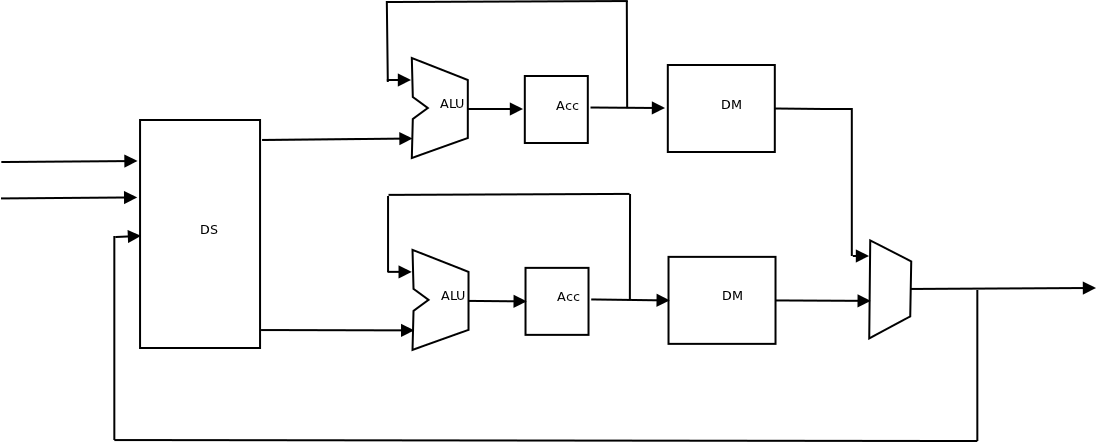
\includegraphics[width=0.8\textwidth]{images/new_path}
	\end{center}
	\caption{A block diagram of the modified area of the leros data path. ACC is the accumulator, DM is the data memory, DS is the data select}
	\label{new_path}
\end{figure*}

The use of a 4 bit memory address operand limited the maximum number of additional ALUs to 32. A limit was also imposed by the board used as it only contained 36 blocks of ram meaning that even if a larger operand had been used little extra performance would be gained. This meant that the board’s memory was again acting as the bottle neck for the design as with the exception of memory the FPGA contained space to synthesise several hundred ALUs and this was the original intent. The only option available at this point however to improve the memory was to use flip-flops instead of the ram. This was highly undesirable for two reasons. Firstly the number of flip-flops that were possible was only around 10,000, while more than enough for most applications when being used as memory this was insufficient for the image processing operations for which the CPU was intended. Secondly the use of flip-flops rather than the on board memory meant that the maximum clock speed of the CPU was reduced by around 50\%. Because of these issues the implementation with a limit of 32 ALUs was kept.

The movement of data between memory blocks meant that while the CPU could perform the arithmetic and logical operations in parallel its memory operations could only occur in serial and due to the need to move data between memory blocks a significantly higher number of these load and store operations would be required for the program to perform. How much this affected the speed up of the additional ALUs would be largely program dependent. 

The implementation of several other instructions required alteration to work with the new multiple ALUs. The add and load immediate operations were altered to allow the immediate to be placed on the bus to all the ALUs so that they all performed the operation. All the branching and jumping operations operated only on the first ALU with this ALU being the only one to contain the branch flag registers. This was done as with a single control unit the ALUs all had to perform the same instructions and so could not branch to different sections of code.